\documentclass[twocolumn,9pt]{article}
\usepackage{amsmath}
\usepackage{graphicx}
\usepackage{color}
\usepackage{citesort,natbib}
\usepackage{longtable}
\usepackage{tabu} %% text tables
%%\usepackage[linktocpage=true]{hyperref} %% links to numbers instead of sections
\usepackage{hyperref}
%%\usepackage{url}
\usepackage[small,compact]{titlesec}
%\usepackage{geometry}
%\geometry{left=3.5cm,right=3.5cm,top=3.5cm,bottom=3.5cm}
%\graphicspath{{./WP_images/}}
\usepackage{amsmath}
%%\usepackage{cite} 
%%\usepackage{notoccite}
\usepackage{xspace}
%\usepackage[backend=bibtex,sorting=none]{biblatex}

\newcommand{\bat}{\textsf{BAT}\xspace}

\makeatletter
\def\@maketitle{%
  \newpage
%  \null% DELETED
%  \vskip 2em% DELETED
  \begin{center}%
  \let \footnote \thanks
    {\LARGE \@title \par}%
    \vskip 1.5em%
    {\large
      \lineskip .5em%
      \begin{tabular}[t]{c}%
        \@author
      \end{tabular}\par}%
    \vskip 1em%
    {\large \@date}%
  \end{center}%
  \par
  \vskip 1.5em}
\makeatother


\begin{document}
\sloppy
\title{%
Toward Putting Advertising Transactions on the Blockchain\\[1mm] 
\normalsize \bf Re-inventing Digital Advertising with the Basic Attention Token (\bat) }
\author{Anonimized for Submission\footnote{To be used for review purposes. Please do not distribute.}}
\date{}
\maketitle

\begin{abstract}
Digital advertising is broken. The marketplace for online advertising, once dominated by advertisers, publishers, and users, has by now become overrun by ``middlemen:'' ad exchanges, audience segmentation, complicated behavioral and cross-device user tracking, and opaque cross-party sharing through data management platforms. 
Users today face unprecedented levels of malvertisement~\cite{malvertising}, and privacy violation. 
Moreover, advertising slows browsing down, especially on mobile devices; further, mobile advertising results in as much as~\$23 per month in data charges on the average user's data plan, slow page loads, and as much as~21\% less battery life.  
In response, over~600 million mobile devices and desktops (globally) employ ad blocking software and this number is growing~\cite{blocking,blocks-ads}. 
%%This crisis for traditional publishers is now exacerbated by the rise of Google and Facebook, which together claim 73\% of digital ad revenue and 99\% of all growth. 

Traditional publishers have lost approximately~66\% of their revenue over the past decade, adjusted for inflation. 
Publishers lose billions of dollars to increasing levels of fraud and faulty means of attributing user attention. 
Publishers face falling revenue, users feel increasingly violated, and advertisers' ability to assess effectiveness is diminished. 
The solution is a decentralized, transparent digital ad exchange based on Blockchain. 
The first component is \href{https://www.brave.com}{Brave}, a fast, open-source, privacy-focused browser that 1)~blocks third party ads and trackers; ~2)~implements a \emph{ledger} system; and that 3)~measures user attention to reward publishers. 

The Brave web browser introduced the \bat (Basic Attention Token), a token for a decentralized ad exchange. It compensates the browser user for attention while protecting privacy.
\bat connects advertisers, publishers, and users and is denominated by relevant user attention, while removing social and economic costs associated with existing ad networks, e.g., fraud, privacy violations, and malvertising.
\bat is a payment system that rewards and protects the user, while giving better conversion rates to advertisers and higher yield to publishers.
We see \bat and associated technologies as part of future web standards, solving the important problem of monetizing publisher content, while simultaneously protecting user privacy. 

\end{abstract}

\section{Basic Attention Metrics (BAM)}
\label{sec-4-1}

To improve the efficiency of digital advertising requires a new platform and unit of exchange. The first phase involves the roll-out of a new browser, Brave, a fast, open source, privacy-focused browser that blocks invasive ads and trackers, and contains a ledger system that anonymously measures user attention to accurately reward publishers. The next phase involves the introduction of Basic Attention Token or \bat. It is a token for the decentralized ad exchange. \bat connects advertisers, publishers, and users, creating a new, efficient marketplace. \bat is an ERC20 Ethereum token. The token is derived from~---~or denominated by~---~user attention. Attention is really just focused mental engagement~---~on an advertisement, in this case.

The ability to privately monitor user interests at the browser level allows for the development of rich metrics for user attention. For example, it is known whether an impression has been served to an active tab, and measure the seconds of active user engagement. Attention is measured as viewed for content and ads only in the browser's active tab in real time. For instance, the attention value for the ad will be calculated based on incremental duration and pixels in view, in proportion to relevant content. %We will define further anonymous cost-per-action models as the system develops.

On-device machine learning can match truly relevant ads to content from a level that middlemen with cookies and third party tracking are unable to achieve, regardless of how much of the user data is extracted and monitored from external models. External models are still unable to track transactions well enough not to serve ads for products users have often already purchased. User engagement through genuine feedback mechanisms ensures that users that have opted in for \bat are getting the best possible product match that they're most likely to lead to convergence. %Ultimately it comes down to trust and respect with and for the user. By keeping the data on the device only, encrypting the data and shielding the identities of our users as a core principle, \bat forms a bond with users that proves that not only does their data hold value, it holds substantial value that has been ignored and exploited by the middlemen year after year in the current model. 

\section{Token Technology}
\label{sec-4-2}

The Basic Attention Token (\bat), an ERC20 token based on Ethereum, is an important element of a new marketplace. Ethereum is an open source, blockchain-based, distributed computing platform oriented towards smart contracts. 
Ethereum has been used for mobile payment systems, distributed exchanges, tokens pegged to commodities and fiat currencies, market clearing mechanisms, micropayment systems for distributed computing resources, commodities and securities exchanges, crowd-funding, and legal document verification. %Large firms have invested in and deployed Ethereum, with JP Morgan, Deloitte, IBM, Santander Bank, Microsoft, the Luxembourg Stock Exchange, and the Royal Bank of Scotland being key early adopters. 
Micropayments using \bat will be accomplished for the first stage deployment with the Brave Micropayments \href{https://github.com/brave/ledger}{Ledger}. Each viewed ad will be verified within the browser using the BAM. 

\section{\bat for User Applications}
\label{sec-4-4}

As users are given access to some of the advertising spend in \bat, they will become an important and active part of the advertising and publishing economy, rather than the passive participants they are presently treated as. While tokens can be donated to individual content providers and publishers, there are a number of use cases for the tokens.

\begin{itemize}\itemsep=-3pt
	\item 
\textbf{Targeted advertising:} An obvious use case is for very specific targeted advertising. Many small businesses have modest requirements which may be well served by tokens they acquire through their normal browsing activities. Users may also find new uses with low barrier to entry highly targeted ads; personal ads targeting people of a religion or subculture for example.
\item
\textbf{Subscriptions:} 
Some publishers may have premium content they would ordinarily only offer to subscribers. Since subscription models are not typically favored by users on the internet, this could unlock new revenue for premium content providers. Content may also be bought for friends using the token; if someone likes a premium article, they can make a micropayment to send it to three of their friends.
\item 
\textbf{Differentiated content quality:} 
Higher quality content may also be offered to users for a \bat transaction. For example, higher quality video or audio on an entertainment channel, or some kind of summary of headlines in a news source. Video or audio content in a news or other information source may be restricted to people who pay a small micropayment.
\end{itemize}

%\begin{figure}
%\begin{center}
%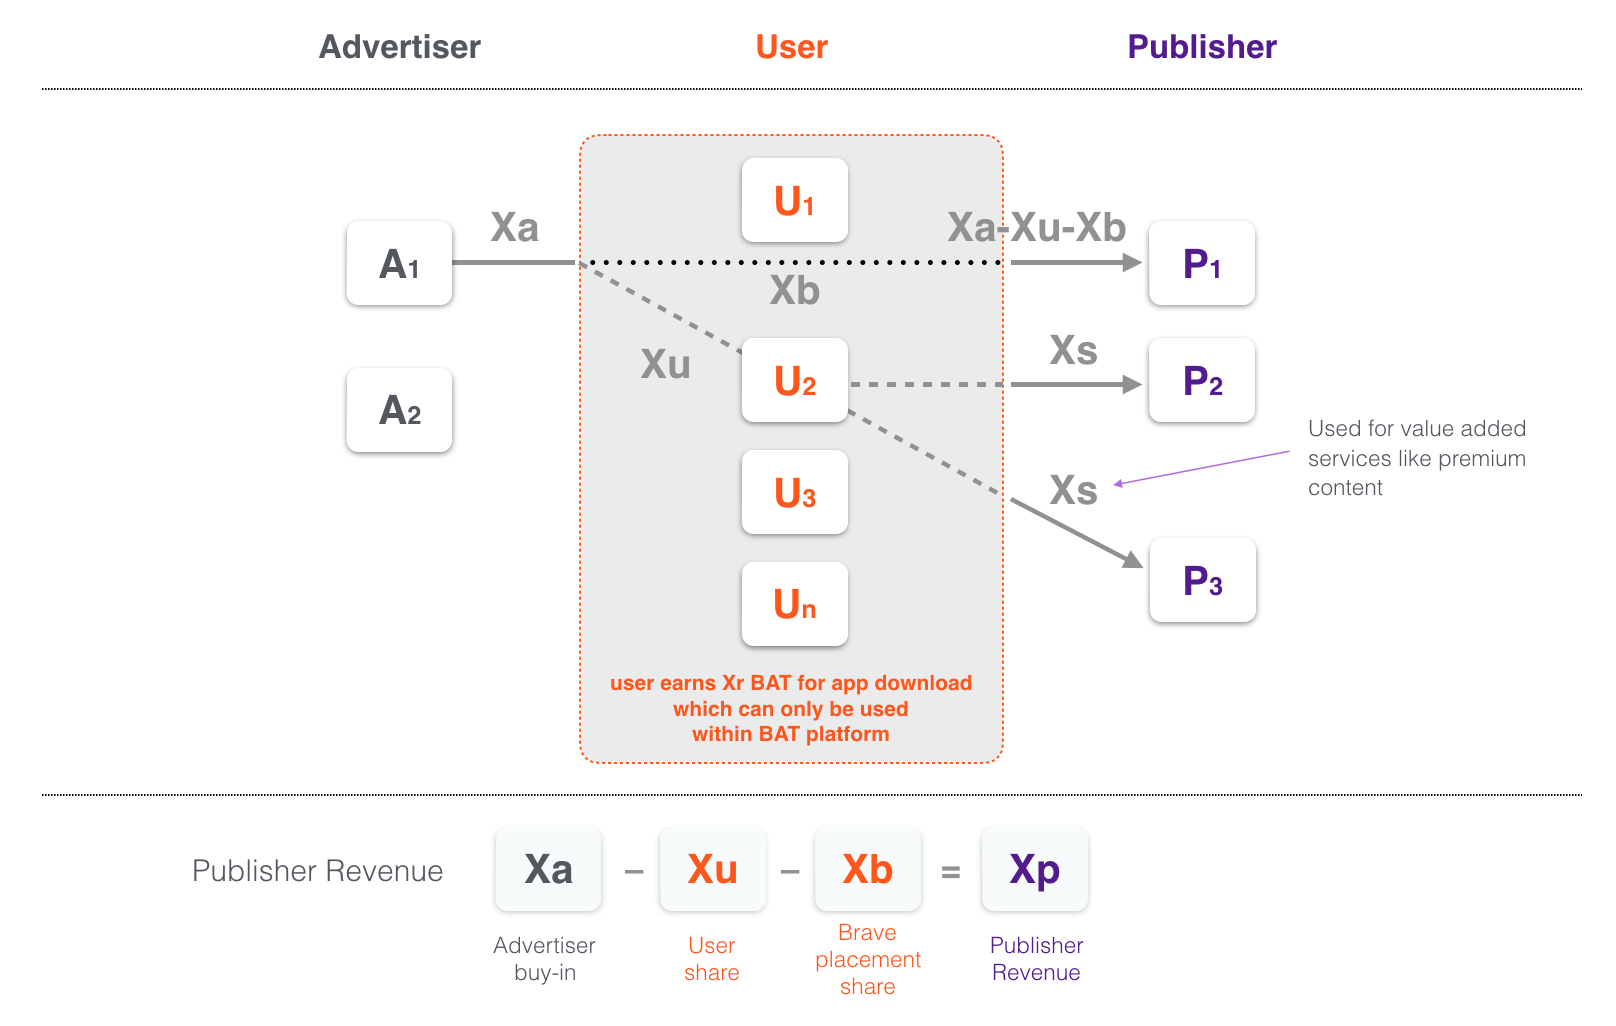
\includegraphics[width=\columnwidth]{BAT_tokentech_diagram.png}
%\caption{Value Flow of the Basic Attention Token}
%\end{center}
%\end{figure}

%This flow shows the conceptual flow of the \bat payments. The flow of the \bat payments will not follow this chart precisely in first iterations of the \bat payment system as the payments will be regulated by the Brave ledger system, but the total effect will be the same. The high-level concept is the advertiser sends a payment in token along with ads to users in a locked state Xa. As the users view the ads, the flow of payments unlocks, keeping part of the payment for their own wallet (Xu), and passing on shares of the payment to Brave (Xb) and passing the remainder on to the Publisher (Xa-Xu-Xb).  
\noindent
\bat will, in early stages, be tied to Brave browsers and Brave servers, along with verified publishers. Ad fraud will be prevented or reduced by publication of source code, rate limiting and cryptographically secure transactions. Ads served to individual browser/users will also be rate-limited and tied to active windows and tabs. Payments in \bat will be sent only to publishers, though a payment for viewing an ad on one publisher may be used at another publisher or kept for some other premium services supplied through the \bat system.

\section{Micropayment System for \bat}
\label{sec-4-3}

\newcommand{\point}[1]{\smallskip\par\noindent\textbf{#1.}~}

\bat is enabled by a Ethereum-based micropayment system~\cite{bolt,decentralized-anonymous,McCorry2016,Miller2017}. While there is quite a bit of related work in this space, of course, deployment at scale is different from deploying an algorithm or a technology within a research prototype.
The challenges of deploying such a system are three-fold, as detailed below. 

\subsection{Scalability} 
The \bat micropayment system needs to be able to process millions of transactions a second, when fully operational. State channels allow for multiple small transactions with strong anonymity guarantees when using the correct matching algorithms. While Raiden and other state channel schemes are becoming integrated with the Ethereum ecosystem, and new blockchains such as Zcash and Monero offer stronger privacy guarantees, along with rapidly increasing feature sets, it is likely that a new scheme addressing the unique problems of this type of transaction will be used for large scale multiparty transfer of \bat.
%\point{Practical challenge} 
It remains to be seen what exactly needs to appear on a (public) ledger and what will be relegated to payment/state channels. 

\subsection{Privacy} 
Given that many transactions will be available on a public blockchain, the system needs to protect the anonymity of the users.
The Brave Ledger system, which is an open-source Zero Knowledge Proof scheme, presently deployed to allow Brave browser users to make anonymous donations to publishers using \bat as the medium of exchange. The Brave Ledger system uses ANONIZE~\cite{anonize} to protect user privacy, to break the link between individual users and the aggregate payments to publishers. 

A lottery system may be used, where small payments are made probabilistically, with payments happening essentially in the same way that coin mining works with proof of attention instead of proof of work~\cite{micropayments,decentralized-anonymous}, BOLT~\cite{bolt}, Zero Knowledge SNARK or zkSNARKs~\cite{Reitwiessner2016} algorithms may become part of this stack for guarding privacy of participants. The \bat situation is mitigated by the fact that the privacy of the browser customer is of primary importance; publishers and advertisers have fewer privacy concerns. 
Still, while privacy of advertisers and publishers is not our highest priority, advertisers and publishers might not want to share information about either their bids or money exchanging hands with each other, because doing so would compromise their established business practices. How to combine these goals with integrity remains to be seen and may involve the use of mechanisms such as zkSNARKs~\cite{Reitwiessner2016}, as mentioned above.
Of course, deployment in a web browser brings with in a significant number of challenges such as tracking.%, cookie exchanges, etc.

\subsection{Integrity}
The deployed system needs to provide assurances to both advertisers and publishers that they are not cheated through either accounting tricks, bots, or click-jacking and are properly compensated. 
A fully distributed ledger is desirable, both for public accountability and potential scalability reasons. Publishers, advertisers and users of the \bat token will have incentive to use such a system to keep track of payments within the \bat system. 
How to balance the integrity and privacy demands of individual participants remains to be seen. 
%\point{Practical challenge} 

\section{Conclusions}
As the Brave browser moves to a fully distributed micropayment system, we expect other developers to use our free and open source infrastructure to develop their own use cases for \bat. 
We want \bat and the tools associated with it to eventually become important web standards for future development of web content. 
Publishers, advertisers, and users deserve a private, secure and well-engineered future.

{
\setlength{\bibsep}{0pt plus 0.3ex}

\footnotesize
\bibliographystyle{plain}
\bibliography{berkeley}
}
\end{document}
